\documentclass[11pt]{article}

\usepackage{times}
\usepackage[utf8]{inputenc} % allow utf-8 input
\usepackage[T1]{fontenc}    % use 8-bit T1 fonts
\usepackage{url}            % simple URL typesetting
\usepackage{graphics}
\usepackage{color}
\usepackage{amsfonts}       % blackboard math symbols
\usepackage{amsmath}       % blackboard math symbols
\usepackage{amssymb}
\usepackage{multicol}
\usepackage{enumerate, multirow, color, graphicx, lastpage, listings, tikz, pdflscape, subfigure, float, polynom, tabularx, forloop, geometry, listings, fancybox, tikz, forest, tabstackengine, cancel}

\graphicspath{{../graphics/}}
\usepackage{geometry}
\geometry{left=2.8cm,right=2.8cm,top=2.6cm,bottom=2.6cm}
\usepackage{fancyhdr}
\pagestyle{fancy}
\usepackage{hyperref}% should be the last package you include

\newcommand{\theteam}{}
\newcommand{\team}[1]{\def\theteam{#1}}


\fancyhead[L]{\rightmark} % I changed this from : \fancyhead[L]{\theteam} (think it is just less ugly like that)
\fancyhead[R]{\thepage}
\cfoot{}

\setlength{\parindent}{0pt}

% For tighter image bounds and caption bounds
\setlength{\belowcaptionskip}{-10pt}
\setlength{\abovecaptionskip}{-10pt}
\setlength\intextsep{0pt}

\team{Jessica Bader, 5624582; Philipp Noel von Bachmann, 4116220 }
\title{Extremely Lossy Compression through Reinforcement Learning}
\author{\theteam}

\DeclareMathOperator*{\argmax}{arg\,max}

\begin{document}
\maketitle

\begin{multicols*}{2}
\section{Introduction}



\section{Related Works}
\section{Methods}

\subsection{Architecture}\label{methods:Architecture}
    In Deep-Learning based compression, encoding comprises of the data first
    beeing transformed by a neural network into a latent space. Then this latent
    space is losslessly encoded and transmitted. On the decoding side, the
    latent space is decompressed and passed through another neural network back
    to the input domain.

    \begin{figure}[H]
        \centering
        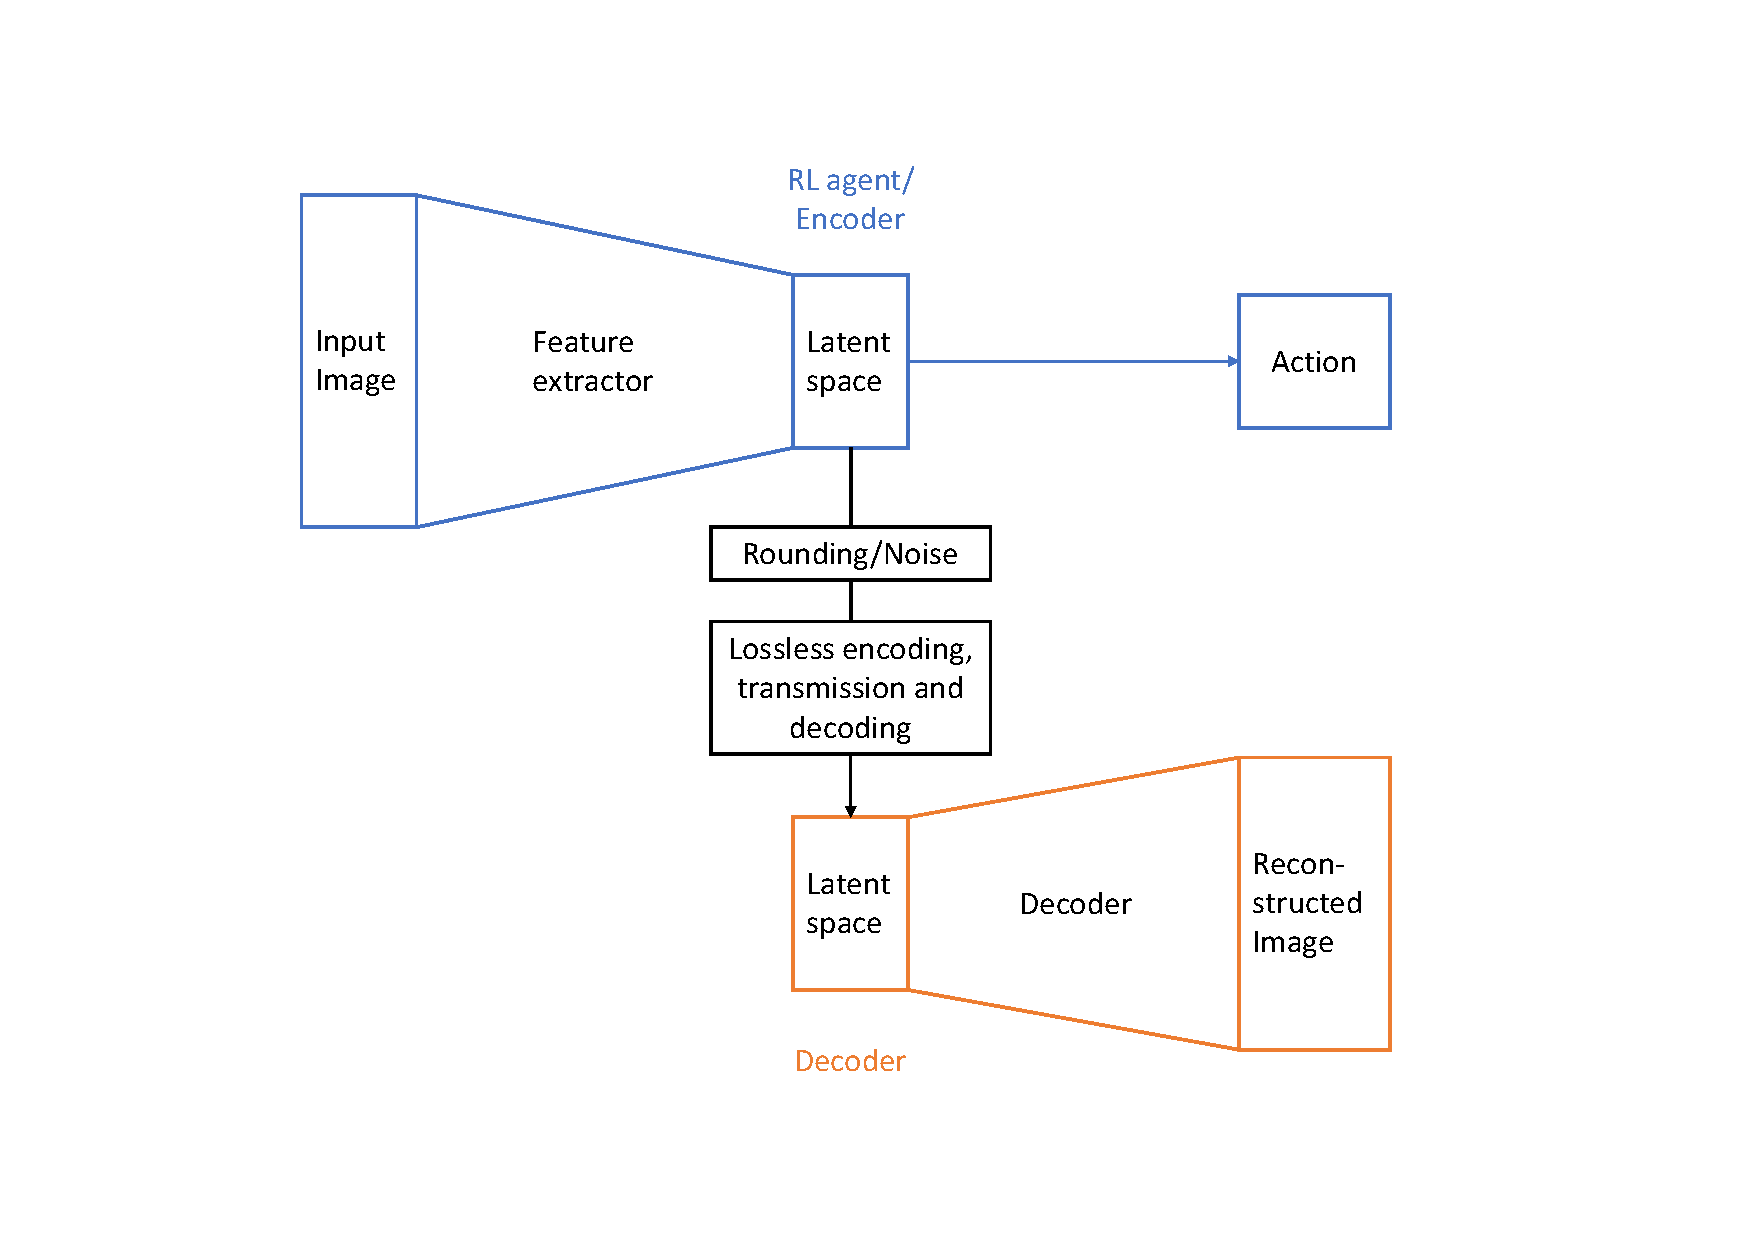
\includegraphics[width=0.8\linewidth]{images/architecture.pdf}
        \caption{Overall architecture. First, the input image gets transformed by the feature extractor to the latent space. The latent values get rounded/noise gets added. Then the values get losslessly transmitted. Finally the decoder tries to reconstruct the input image from the latents.}
        \label{fig:Architecture}
    \end{figure}

    In our approach, a Reinforcement Learning agent takes the place of the first
    neural network. The agent contains a so-called feature extractor, which
    extracts features from the observation that are important for determining
    the action. As described in ??, this information should also be important
    for reconstruction. Then the latent space is losslessly encoded and
    transmitted with an algorithm of choice (for example ..., for training this
    step is not strictly necessary as the latents get losslessly decompressed in
    the next step). After decoding the latents they are passed through the
    second network which in this case is a normal upsampling CNN (TODO: which name??).
    Figure \ref{fig:Architecture} shows an overview of the architecture.

\subsection{Theory}
    Lossy compression trades between having a low bitrate and a low distortion.
    This section describes the theory of these objectives applied to our
    problem.\newline

    To determine the bitrate of an algorithm, one has to look at the encoding
    process of the data, where the data gets mapped from the input image to the
    latent space, see \ref{methods:Architecture}. The process decreases the
    bitrate compared to the original input image, if the entropy of the latent
    space is lower than the input space, and a sufficiently fitting encoding
    distribution for transmission of the latent values is chosen. If the
    distribution over the latent variable $z$ is given by $Q_\theta(Z=z \vert x)$ where
    $\theta$ parametrizes the distribution and $P(Z=z)$ is used to encode the
    latents, the bitrate is given by the cross entropy
    \begin{equation}\label{eq:BitRate}
        \mathbb{E}_{z \sim Q_\theta(Z=z \vert x)}[log(P(Z=z))]
    \end{equation}
    In addition, the entropy of $Q_\theta(Z=z \vert x)$ gives the case when
    $Q=P$ and we would have the perfect encoding distribution. Therefore the
    entropy gives a lower bound on the cross-entropy.

    As neural networks have real valued outputs which means that $Q_\theta(Z=z
    \vert x)$ is a continuous pdf, the bitrate is very high. Therefore one
    approach is to round the latent values. This reduces $Q$ to a discrete
    probability distribution, which reduces the cross entropy. However, rounding
    is a undesirable operation during training, since the gradient of the
    rounding operation is 0 nearly everywhere. Therefore, we replace the
    rounding during training by the addition of uniform noise $u$, see also
    figure \ref{fig:Architecture}. The noise addition shifts the values
    similarly to rounding, but is differentiable.

    Another effect of adding uniform noise is that we can reparametrize
    \ref{eq:BitRate} and take the expectation over the uniform noise:
    \begin{equation}
        \mathbb{E}_{u \sim U[-\epsilon, \epsilon]}[log(P(Z=\hat{z} + u))]
    \end{equation}
    where $\hat{z}$ is the mean of $Q_\theta(Z=z \vert x)$. \newline

    % (To be more precise: We start with a continuous pdf. Rounding creates a
    % bunch of delta pulses which are nondifferentiable. However we can
    % approximate the continuous pdf by adding uniform noise to the new discrete
    % pdf. Therefore we can also just add noise instead of round?)


    % In turn, this means that the encoding network shouldn't encode information
    % in small differences. One approach to achieve this behaviours is to add
    % noise to the latent values, which forces the RL-agent to get more robust to
    % noise.

    % [TODO: this part is just disregared in balle]
    The encoding distribution $P$ is naively chosen to be a normal distibution. The
    mean can be chosen arbitrary given a powerful enough transformation, so it is
    set to 0 for simplicity. The variance gets learned during the training process.


    Decreasing the bitrate is often traded against an increase in distortion.
    Therefore we need a performance measure to evaluate the distortion of the
    reconstructed image $\hat{x}$. A traditional metric is the Mean Squared Error (MSE),
    \begin{equation}\label{equ:L2}
        \mathbb{E}_{x, \hat{x}}[\sum_{i,j} (x_{ij} - \hat{x_{ij}})^2]
    \end{equation}
    If humans look at images however, they often just care about specific types
    of distortion. A slightly lower brightness for example wouldn't matter for
    most images, but probably a different colour or more generally they care
    more about semantic distortion that would give them a different
    interpretation and representation of the image. MSE however gives these
    distortions all the same values.

    As the RL-Agent is used to encode the data and therefore should extract the
    relevant features, it seems reasonable to let the agent also judge the
    reconstruction. Therefore, a second approach will be to compare not the
    original image and the reconstuction, but rather the agents representation
    of the images to measure similarity. In practive, this means passing both
    images through the feature extractor and measuring the L2 distance in latent
    space.







% \subsection{Objective function from view of variational inference}
%     In Lossy image compression, the objective function is given by the ELBO:
%     \begin{align}
%         & \mathbb{E}_{z \sim Q(Z= z)}[log P(X, Z= z) - log Q(Z = z)]\\
%         & = \mathbb{E}_{z \sim Q(Z= z)}[log P(X \vert Z= z) - log \frac{Q(Z = z)}{P(Z = z)}]\\
%         & = \mathbb{E}_{z \sim Q(Z= z)}[log P(X \vert Z= z)] - D_{KL}[Q(Z = z)\Vert P(Z = z)]\\
%     \end{align}

%     Problem is, that we cannot differenciate by q since expectation is over q,
%     so just fix q by uniform distribution, and do reparametrization trick

%     now entropy of q becomes fixed so we can remove from optimization, just need
%     to care about $E_U[P(Z + U)]$

%     just need to choose encoding distribution, choose naively as normal with
%     mean 0 and learned variance since needs to be flexible.

%     for likelihood, choose normal (leads to MSE) and fix variance

\subsection{Training}
    RL-agents are normally trained with a specific loss function, which will be
    abstracted by $Loss_{RL}$. As the RL-agent takes the role of the encoder, it
    is responsible for the bitrate. Therefore we add the loss from
    \ref{eq:BitRate} to the standard loss:
    \begin{equation}
        \mathbb{E}_{x}[Loss_{RL}(x) + \alpha\cdot \mathbb{E}_{u \sim U[-\epsilon, \epsilon]}[log(P(Z=\hat{z} + u))]]
    \end{equation} where $\alpha \in \mathbb{R}$ is chosen to balance the two terms.
    Both expectations will be approximated by empirical means over the training
    data. As the RL-agent is independent of the decoder, we can also train it
    separatly first.

    After training the RL-agent, we fix its values. Therefore at this point, the
    encoding to the latents is fixed. Now the decoder to get the reconstruction
    needs to be trained. For the decoder, we use the L2 loss given in \ref{equ:L2}/ we use the loss functions discussed in \ref{sub:Decoder_Loss}

\subsection{Decoder loss}\label{sub:Decoder_Loss}
    For our decoder, we tried several loss functions. The simplest version was
    the MSE between the original and reconstructed images. \\
    In early experimentation (see section 4.1), we found that some details which
    may be considered important to the task, specifically the location of the
    ball, were omitted as they accumulated little MSE penalty; in an attempt to
    recover these aspects, we devised a second loss scheme, which we refer to as
    latent loss. The motivation was to reward the decoder for reconstructing the
    image in such a way that the same features would be extracted, resulting in
    preserving the most important aspects. For this loss, we passed the
    reconstructed image through the feature extractor and evaluated the MSE
    between the original latent space and the reconstructed latent space.

\subsection{Adaptive alpha (omitted)}
During training, an issue arose in choosing $\alpha$ (see Experiments and Evaluation) which we believe was caused by the RL reward: the agent behaves randomly in early iterations and earns little reward, but this improves drastically once it has started learning. Therefore, choosing $\alpha$ too large prevents the agent from ever learning to complete the task, while choosing $\alpha$ too small allows the agent to ignore the cross entropy loss while fine-tuning its actions. We tried to resolve this with a non-static $\alpha$: as the reward grows, the relative importance of the two terms should stay approximately the same. We designed several adaptation schemes (others can be found in Future Work), but the general algorithm we chose was to update $\alpha$ each time the ratio threshold was violated. We implemented this by
\begin{equation}
    \alpha = \alpha \cdot 10 \cdot e^{-i / 1000}
\end{equation}
where $i$ is the number of iterations. Multiplying by the negative iterations ensures that $\alpha$ changes most drastically at the beginning, but will converge over time.
\section{Experiments and Evaluation}
TODO: dataset
\subsection{Dimension reduction}
Our first set of experiments featured the basic dimension reduction method,
without the modifications for compression. We were looking to verify that the
required reconstruction information was present within the lower dimensional
representation created by the feature extractor. (TODO include bitrate) The
qualitative results can be seen in Figure 1. \\

We also utilized our latent loss scheme by pre-training on image reconstruction
before training on the latent loss. The results can be seen in Figure 2.
\begin{figure}[H]
    \centering
    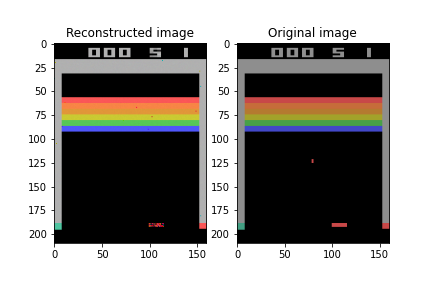
\includegraphics[width=0.6\textwidth]{images/orig_reconstructed0.0.png}
    \caption{Baseline method (no compression) with decoder trained on MSE for 10,000 iterations}
    \label{fig:baseline_MSE}
\end{figure}
\begin{figure}[H]
    \centering
    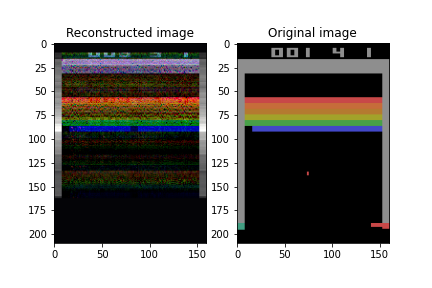
\includegraphics[width=0.6\textwidth]{images/orig_reconstructed_rl3.0.png}
    \caption{Baseline method (no compression) with decoder trained on MSE for 10,000 iterations, then latent MSE for 10,000 iterations}
    \label{fig:baseline_MSE_latent}
\end{figure}

\subsection{Compression}
Now we added the compression loss to the training of the RL agent
\ref{eq:RL_Training_Loss} and trained the agent with this loss function. We
modified the $\alpha$ value, the idea beeing that larger alpha values give a
larger penalty and therefore higher compression. Ultimatly however, the
performance of the Encoder together with the Decoder is important, a too high
compression would destroy too much information. %TODO: That is true but alpha in our case wasnt stabely changing compression performance

An alpha of $1e-8$ TODO: verify seemed to work best for the Decoder, therefore
we chose this value for an extended run over ... TODO: add epochs. Tested on an
independently created test dataset, this resulted in an entropy of 1.7 bits per
latent dimension, if the latent values get rounded to 3 digits. The actual
bitrate given as the cross-entropy \ref{eq:BitRate} is higher however, since
we need to choose a fixed distribution for encoding and transmission of the
latents. As for training we chose a normal distribution with mean 0 and learned
variance, we also use this for testing. The expected variance per dimension was
estimated by the mean per dimnesion over the whole test dataset. However the
cross entropy over the test dataset was infinity. A visual investigation of the
latent values showed that while the entropy of the latent values was low, some
of the values deviated of 0 significantly, (in the order of 100), which led to a
probability of nearly 0 and a logprob of -infinity.

After training the RL Agent, the decoder was trained for ... TODO: add epochs.
This resulted in an MSE Loss of 1895 or 2322 ?? TODO. As discussed in
\ref{sec:Introduction}, MSE Loss is not a good metric for performance, since it
gives each pixel the same value. Therefore we investigated some images. An
example can be seen in figure \ref{fig:final_agent}. The image shows that during
compression some of the data got lost, since the image is distorted.
\begin{figure}[H]
    \centering
    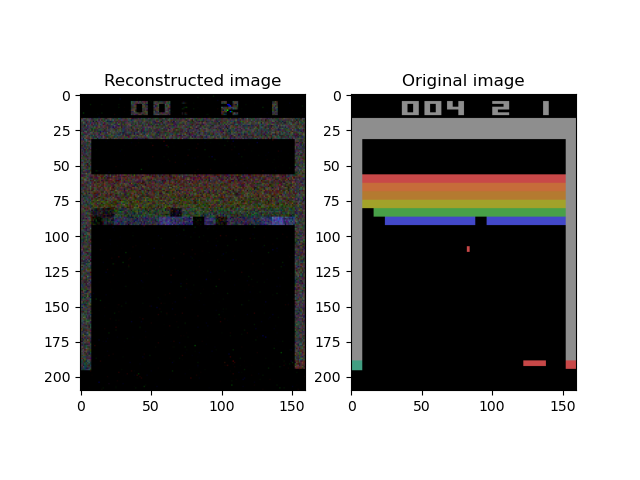
\includegraphics[width=0.6\textwidth]{images/orig_reconstructed_final_agent.png}
    \caption{Baseline method (no compression) with decoder trained on MSE for 10,000 iterations}
    \label{fig:final_agent}
\end{figure}

\subsection{Adaptive Alpha}
When we implemented our custom loss function with static $\alpha$, several
rudimentary tests were done to verify that the model behaved as expected. One
such test involved varying $\alpha$: we expected that a lower value would
prioritize task performance, while a higher value would prefer a lower bitrate.
However, we found this was not the case: there seemed to be just as much
variation between independent tests of the same $\alpha$ as changing $\alpha$
(add results in appendix?). Given our hypothesis for where the problem lay (see
Methods), we developed the adaptive $\alpha$ scheme. However, initial results
showed no improvement and we were forced to move this to Future Work.

\subsection{Pretrained agents}
Another idea was that maybe adding the compression loss to the RL agent from the
beginning on was a too large constrain for the agent to learn anything.
Therefore, we tried to fix this by first pretraining the agent, and then adding
the compression loss to the agent. On the one hand, the compression loss reduced
the entropy but on the other hand, the decoder couldn't learn anymore, so this
procedure showed no improvements.




% TODO:

% structure eval:
% - show compression performance, maybe the curve
% - show that while entropy is low, cross entropy still high for final agent (overfit?)
% - show some images during training, agent can learn paddle position, not only memorize images
% - show that it breaks down for evaluation set

% other experiments:
% - github code: scaled noise together with variance
% - write up pretrained agent that was trained on, but info just destroyed


\section{Discussion/Future Work}
As can be seen in Figure 1, our baseline with the image MSE produced encouraging
results: the location of the paddle was consistently preserved. However, areas
of improvement include the artifacts that exist in this paddle along with the
loss of the ball.
%  As seen in Figure 2, use of the latent loss scheme resulted in
% extreme artifacts, as well as the loss of the paddle and did not result in ball
% recovery. A new scheme would be needed.\\
\subsection{Bitrate inconsistency}
When adding the custom loss function to the RL-agent, we saw that we could not verify the desired influence. Increasing $\alpha$ did not necessarily decrease
entropy, but entropy fluctuated strongly between runs. One
reason could be that the RL-agent loss function is quite
unstable in itself. While in some epochs, the agent loss was relatively high, it was fairly small in
other epochs. Therefore, we adjusted $\alpha$
dynamically to achieve to a desired bitrate instead of using a fixed $\alpha$.
However, our adaptive $\alpha$ scheme was largely ineffective in verifying the
expected behavior. Therefore, modifications should be made so both task
accuracy and bitrate increase inversely with $\alpha$, or a theoretical
foundation should found why they do not. This could be possible through other
adaptive schemes (thresholds, static ratios, adaptive ratios, etc.). This may
also require reflection to analyze if this divergence from expected behavior is
driven by mechanisms other than RL loss.
\subsection{Bitrate evaluation}
On the test set, the entropy of the final agent \ref{sub:Results_Compression} is
reasonably small and the image is compressed. However, if in testing we encode
the latents with a Normal distribution as during the training process, the
bitrate would rise. This means that while the agents is able to
compress the data, it is not able to fit the distribution.
Therefore future work needs to either fit the agent better to the data or find
a new method to chose/estimate the latent encoding distribution.

\subsection{Decoder generalization}
On the decoder side, we saw that the image quality decreased in
comparison to the baseline, especially on the test dataset. Although a decrease can
be expected due to compression, the decoder failed to reconstruct important
properties like the paddle position, and just reproduced static properties like
the game frame. While we cannot yet rule out insufficient training time (due to
lack of resources), we believe this comes from lack of information in the
encoding. As the encoding is designed to allow the agent to act, it may not be
injective; hence, many different game states could have the same representation. A
new architecture is required, for example: using an earlier layer of the feature
extractor as the encoding; training the encoder and decoder together; using a different encoder
altogether.

\subsection{Latent loss scheme}
Changing the decoder loss function to our latent loss scheme showed no
improvement. The image becomes noisy and information is distorted. Even
in the lower part of the image where normally the screen is black, the decoder introduces noise. One reason for this behaviour
could be similar to adversarial attacks: the decoder tricks
the encoder into generating the desired latents from totally different input images. One improvement could be to combine the latent loss scheme with $L_2$-Loss
such that $L_2$-Loss preserves the general image quality and penalizes distortion,
and latent loss preserves semantic information.

\subsection{Environment}
Furthermore, we would like to explore other environments. Because this
environment included a static start position and relatively slow image change,
we found that many of the images looked similar (full or almost full block
pattern) which lead to overfitting and consqeuently
poor generalization. Using the agent long enough to train and collect diverse
images proved infeasible under time/resource constraints.

\subsection{Train test separatation}
In addition, a unique issue with train/test separation resulted from the
cross-domain approach. Clear separation is an industry standard for data
compression. However, RL agents train freely, and therefore it is not
possible to make guarantees in advance about training images. Our solution was to generate the test dataset independently from our agent,
so that the probability of the same image appearing in both testing and training
was low. Evaluation of this probability would need to be done before this could
be a solution, but is likely intractable as state probabilities are unequal. A
better solution would be to generate a large test set in advance and remove
images if they appear during training. It can also be noted that full, final
results should be reported on a test set rather than a training set (as done in
the section \ref{sub:Dimension_reduction} of experiments). These were done as rudimentary
sanity checks, and were included due to lack of better results.
\section{Questions}
For further questions about this work (including code, omitted results, etc), please contact the authors at jessica.bader@student.uni-tuebingen.de.    
\end{multicols*}

\bibliographystyle{abbrv}
\bibliography{tex/06_Literature.bib}

\end{document}
